\documentclass[tikz]{standalone}
\usetikzlibrary{positioning}
\usepackage{amsmath}
\usepackage{mathrsfs}

\newcommand{\cat}[1]{\mathscr{#1}}
\newcommand{\obj}[1]{\lowercase{#1}}
\newcommand{\objs}[1]{#1}
\newcommand{\mrp}[3]{{#1}:{#2}\to{#3}}
\newcommand{\mrps}[3]{#1(#2,#3)}
\newcommand{\id}[1]{\mathrm{id}_{#1}}
\newcommand{\op}[1]{{#1}^{\mathrm{op}}}
\newcommand{\set}{\mathbf{Set}}
\newcommand{\Top}{\mathsf{Top}}
\newcommand{\blat}{\mathsf{BLat}}
\newcommand{\stone}{\mathsf{Stone}}
\DeclareMathOperator{\dom}{dom}
\DeclareMathOperator{\cod}{cod}
\DeclareMathOperator{\colim}{Colim}
\DeclareMathOperator{\lan}{Lan}
\DeclareMathOperator{\ran}{Ran}
\DeclareMathOperator{\cone}{Cone}
\DeclareMathOperator{\cocone}{Cocone}


\begin{document}
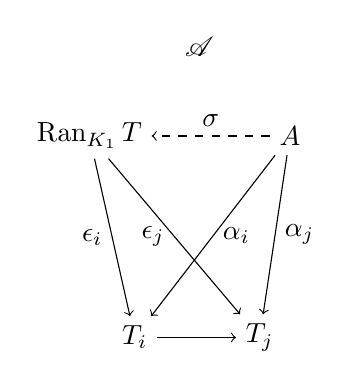
\begin{tikzpicture}
	\node (catA) {$\cat{A}$};
	\node [below left=0.6cm and 0.3cm of catA] (ran) {$\ran_{K_1}T$};
	\node [below right=2.0cm and -0.5cm of ran] (Ti) {$T_i$};
	\node [right=1.0cm of Ti] (Tj) {$T_j$};
	\draw [->] (Ti) to node [above] {} (Tj);
	\draw [->] (ran) to node [left] {$\epsilon_i$} (Ti);
	\draw [->] (ran) to node [left] {$\epsilon_j$} (Tj);
	\node [right=1.5cm of ran] (A) {$A$};
	\draw [->,dashed] (A) to node [above] {$\sigma$} (ran);
	\draw [->] (A) to node [right] {$\alpha_i$} (Ti);
	\draw [->] (A) to node [right] {$\alpha_j$} (Tj);
\end{tikzpicture}
\end{document}
